\documentclass[xcolor=dvipsnames]{beamer}

\usepackage{graphicx}
\usepackage{wrapfig}
\usepackage{colortbl}
\definecolor{myblue}{rgb}{0.8,0.85,1}

\mode<presentation>
{
  \usetheme{Warsaw}
  \setbeamercovered{transparent}
}
% \usecolortheme[named=OliveGreen]{structure}
\setbeamertemplate{navigation symbols}{} 
\setbeamertemplate{blocks}[rounded][shadow=true] 

\title{Asymmetry and the Geometry of Reason}
\subtitle{Causal and Probabilistic Reasoning Conference, LMU M{\"u}nchen}

\author{Stefan Lukits}

\date{June 19, 2015}

\begin{document}

\begin{frame}
  \titlepage
\end{frame}

\begin{frame}
  \frametitle{Epistemic Utility Approach to Justification}
  \begin{figure}[h]
    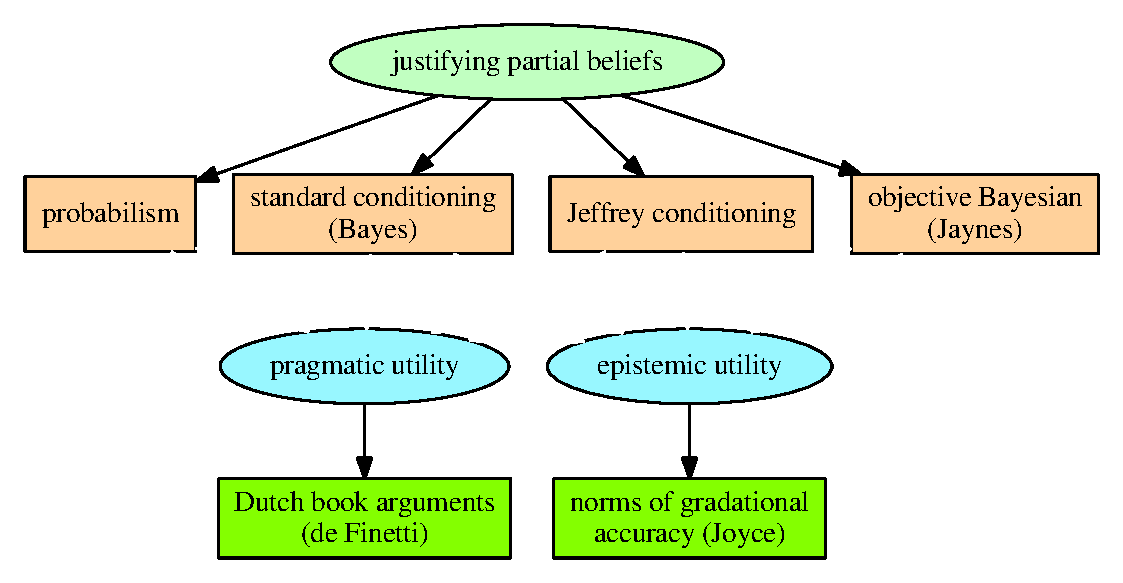
\includegraphics[scale=.6]{./epvspr.eps}
  \end{figure}
\end{frame}

\begin{frame}
  \frametitle{Geometry of Reason vs. Information Theory I}
  \begin{itemize}
  \item \emph{Geometry of Reason:} topology of the probability space is
    metric. A symmetric distance measure is used (Euclidean).
  \end{itemize}
\begin{equation}
  \label{eq:e3}
  \|u-v\|=\sqrt{\sum_{i=1}^{n}\left(u_{i}-v_{i}\right)^{2}}.
\end{equation}
  \begin{itemize}
  \item \emph{Information Theory:} topology of the probability space is not a
    metric. An asymmetric divergence measure is used (Kullback-Leibler).
  \end{itemize}
\begin{equation}
  \label{eq:e7}
  D_{\mbox{\tiny KL}}(u,v)=\sum_{i=1}^{3}u_{i}\ln\frac{u_{i}}{v_{i}}
\end{equation}
\end{frame}

\begin{frame}
  \frametitle{Geometry of Reason vs. Information Theory II}
  \begin{figure}[h]
    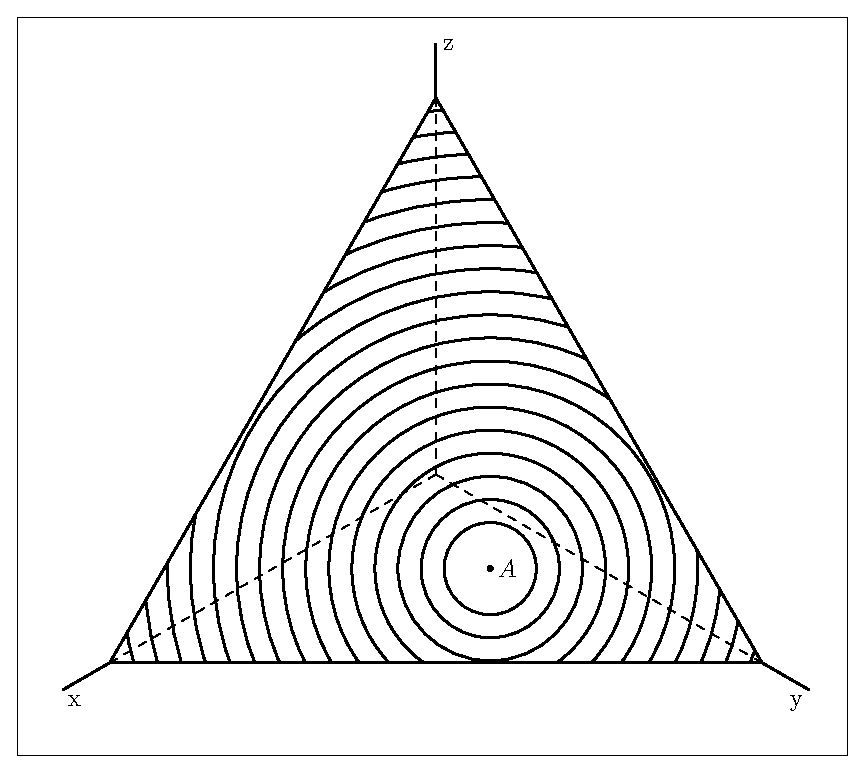
\includegraphics[scale=.6]{./contourslp.eps}
  \end{figure}
\end{frame}

\begin{frame}
  \frametitle{Geometry of Reason vs. Information Theory III}
  \begin{figure}[h]
    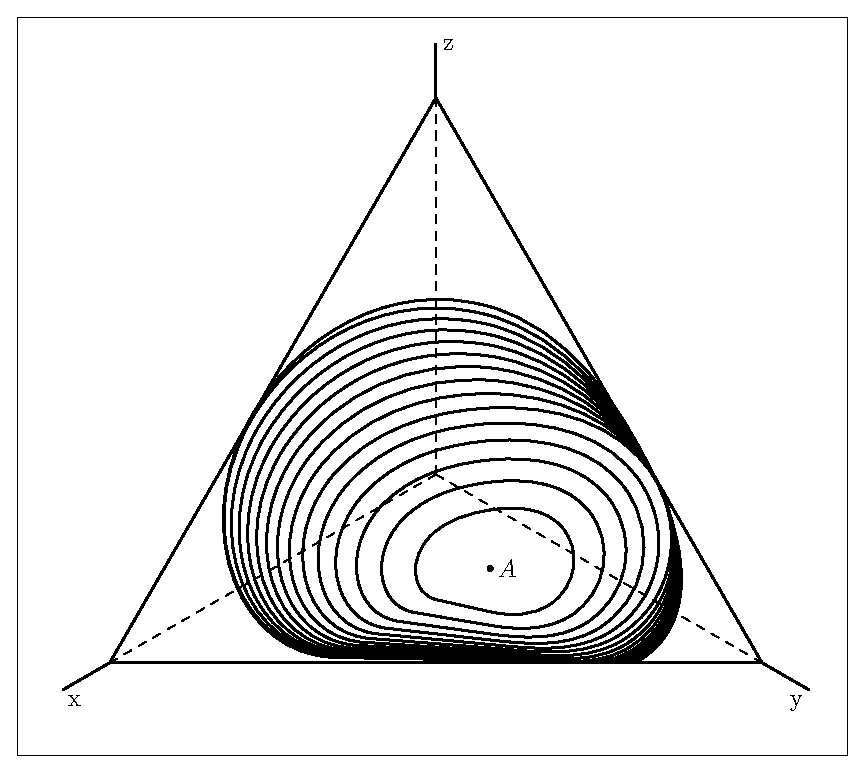
\includegraphics[scale=.6]{./crj.eps}
  \end{figure}
\end{frame}

\begin{frame}
  \frametitle{Weak Convexity and Symmetry}
Here are two axioms for inaccuracy measures which use the language of
the Geometry of Reason (Joyce):
\begin{description}
\item[Weak Convexity] Let $m=(0.5b'+0.5b'')$ be the midpoint of the line
  segment between $b'$ and $b''$. If $I(b',\omega)=I(b'',\omega)$,
  then it will always be the case that $I(b',\omega)\geq{}I(m,\omega)$
  with identity only if $b'=b''$.
\item[Symmetry] If $I(b',\omega)=I(b'',\omega)$, then for any
  $\lambda\in{}[0,1]$ one has\newline
  $I(\lambda{}b'+(1-\lambda)b'',\omega)=I((1-\lambda){}b'+\lambda{}b''),\omega)$.
\end{description}
\end{frame}

\begin{frame}
  \frametitle{Local and Global Inaccuracy}
\emph{Expected local inaccuracy} of degree of belief $x$ in proposition $A$
by the lights of belief function $b$ with respect to local
inaccuracy measure $I$ and over the set $E$ of epistemically
possible worlds:

\begin{equation}
  \label{eq:eli}
  \mbox{LExp}_{b}(I,A,E,x)=\sum_{w\in{}E}b(\{w\})I(A,w,x)=\sum_{w\in{}E}b(\{w\})\lambda\left(\chi_{A}(w)-x\right)^{2}.
\end{equation}

\emph{Expected global inaccuracy} of belief function $b'$ by the lights of
belief function $b$ with respect to global inaccuracy measure $G$
and over the set $E$ of epistemically possible worlds:

\begin{equation}
  \label{eq:egi}
  \mbox{GExp}_{b}(G,E,b')=\sum_{w\in{}E}b(\{w\})G(w,b')=\sum_{w\in{}E}b(\{w\})\mu\|w-b\|^{2}.
\end{equation}
\end{frame}

\begin{frame}
  \frametitle{Standard Conditioning, Jeffrey and LP Conditioning}
  \begin{figure}[h]
    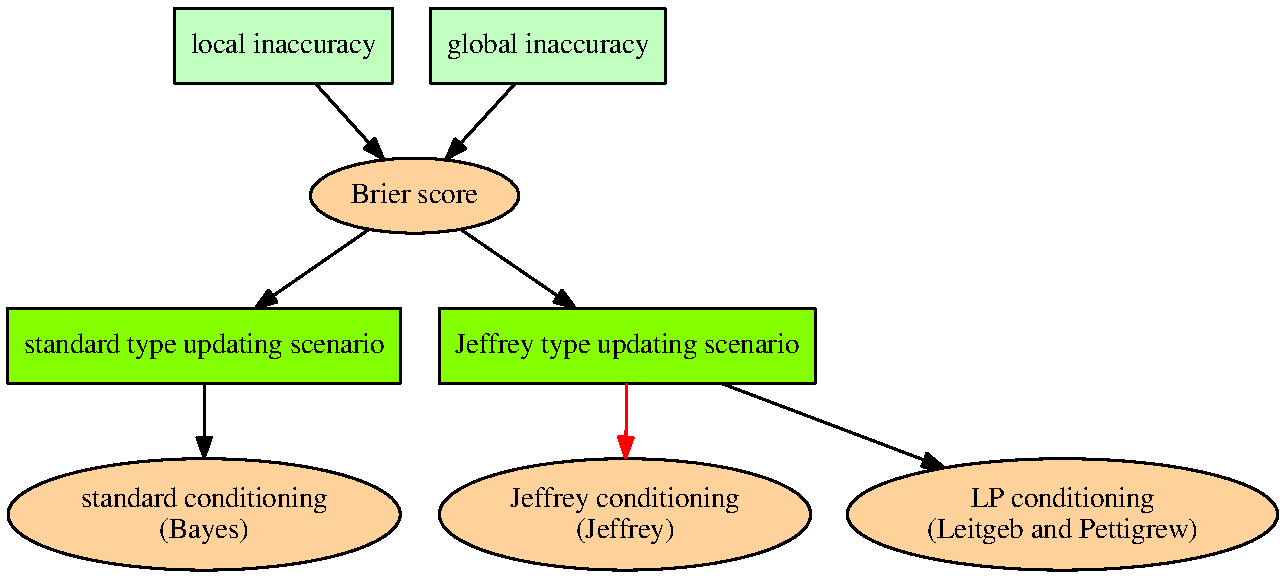
\includegraphics[scale=.5]{./sjlp}
  \end{figure}
\end{frame}

\begin{frame}
  \frametitle{Jeffrey Type Updating Scenario: Priors}
  \begin{figure}[h]
    \includegraphics[scale=.4]{./j1.jpg}
  \end{figure}
\end{frame}

\begin{frame}
  \frametitle{Jeffrey Type Updating Scenario: Jeffrey Posteriors}
  \begin{figure}[h]
    \includegraphics[scale=.4]{./j2.jpg}
  \end{figure}
\end{frame}

\begin{frame}
  \frametitle{Jeffrey Type Updating Scenario: LP Posteriors}
  \begin{figure}[h]
    \includegraphics[scale=.4]{./j3.jpg}
  \end{figure}
\end{frame}

\begin{frame}
  \frametitle{Euclid and Kullback-Leibler}
  \begin{figure}[h]
    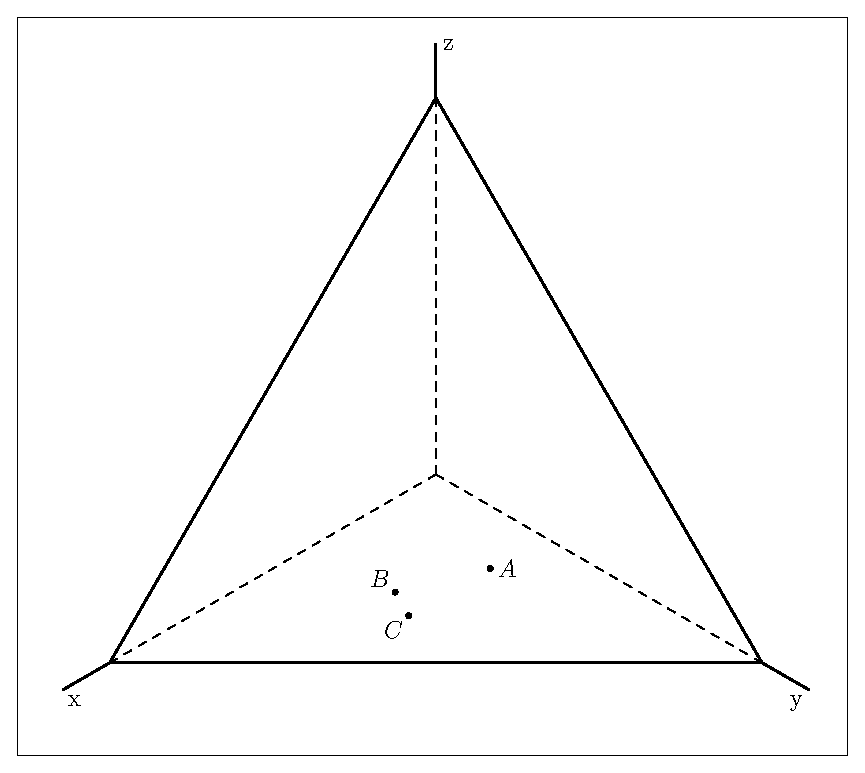
\includegraphics[scale=.6]{./threepoints.eps}
  \end{figure}
\end{frame}

\begin{frame}
  \frametitle{Five Plausible Expectations for an Amujus}
\begin{itemize}
\item \textsc{continuity} An amujus ought to be continuous with
  standard conditioning as a limiting case.
\item \textsc{invariance} An amujus ought to be partition invariant.
\item \textsc{levinstein} An amujus ought not to give ``extremely
    unattractive'' results in a Levinstein scenario
\item \textsc{regularity} An amujus ought not to assign a posterior
  probability of $0$ to an event which has a positive prior
  probability and about which the intervening evidence says nothing
  except that a strictly weaker event has a positive posterior
  probability.
\item \textsc{asymmetry} An amujus ought to reflect epistemic
  asymmetries.
\end{itemize}
\end{frame}

\begin{frame}
  \frametitle{Continuity Violation I}
To illustrate a \textsc{continuity} violation, consider the case where
Sherlock Holmes reduces his credence that the culprit was male to
$\varepsilon_{n}=1/n$ for $n=4,5,\ldots$
\end{frame}

\begin{frame}
  \frametitle{Continuity Violation II}
Straightforward conditionalization on the evidence that ``the
  culprit is female'' gives us 

\begin{equation}
  \label{eq:sherlockcontsc}
  \begin{array}{rcl}
  P'_{\mbox{\tiny SC}}(E_{1})&=&0\\
  P'_{\mbox{\tiny SC}}(E_{2})&=&3/4\\
  P'_{\mbox{\tiny SC}}(E_{3})&=&1/4.
\end{array}
\end{equation}
\end{frame}

\begin{frame}
  \frametitle{Continuity Violation III}
Letting $n\rightarrow\infty$ for Jeffrey conditioning yields

\begin{equation}
  \label{eq:sherlockcontjc}
  \begin{array}{rcccl}
  P'_{\mbox{\tiny JC}}(E_{1})&=&1/n&\rightarrow&0\\
  P'_{\mbox{\tiny JC}}(E_{2})&=&3(n-1)/4n&\rightarrow&3/4\\
  P'_{\mbox{\tiny JC}}(E_{3})&=&(n-1)/4n&\rightarrow&1/4,
\end{array}
\end{equation}
\end{frame}

\begin{frame}
  \frametitle{Continuity Violation IV}
Letting $n\rightarrow\infty$ for LP conditioning yields

\begin{equation}
  \label{eq:sherlockcontlp}
  \begin{array}{rcccl}
  P'_{\mbox{\tiny LP}}(E_{1})&=&1/n&\rightarrow&0\\
  P'_{\mbox{\tiny LP}}(E_{2})&=&(4n-1)/6n&\rightarrow&2/3\\
  P'_{\mbox{\tiny LP}}(E_{3})&=&(2n-1)/6n&\rightarrow&1/3.
\end{array}
\end{equation}

LP conditioning violates \textsc{continuity}.
\end{frame}

\begin{frame}
  \frametitle{Invariance Violation I}
  Consider the Sherlock Holmes scenario. Jane Marple is on the same
  case and arrives at the same relatively prior probability
  distribution as Sherlock Holmes. Jane Marple, however, has a more
  fine-grained probability assignment than Sherlock Holmes and
  distinguishes between the case where Ms.\ S went to boarding school
  with her, of which she has a vague memory, and the case where Ms.\ S
  did not and the vague memory is only about a fleeting resemblance of
  Ms.\ S with another boarding school mate.
\end{frame}

\begin{frame}
  \frametitle{Invariance Violation II}
\begin{equation}
  \label{eq:marpleprior}
  \begin{array}{rcl}
  Q(E_{1})&=&1/3\\
  Q(E_{2}^{*})&=&1/4\\
  Q(E_{2}^{**})&=&1/4\\
  Q(E_{3})&=&1/6.
\end{array}
\end{equation}
\end{frame}

\begin{frame}
  \frametitle{Invariance Violation III}
Now note that while Sherlock Holmes and Jane Marple agree on the
relevant facts of the criminal case (who is the culprit?) in their
posterior probabilities if they use Jeffrey conditioning,

\begin{equation}
  \label{eq:sherlockposteriorjc}
  \begin{array}{rcl}
  P'_{\mbox{\tiny JC}}(E_{1})&=&1/2\\
  P'_{\mbox{\tiny JC}}(E_{2})&=&3/8\\
  P'_{\mbox{\tiny JC}}(E_{3})&=&1/8
\end{array}
\end{equation}
\end{frame}

\begin{frame}
  \frametitle{Invariance Violation IV}
\begin{equation}
  \label{eq:marpleposteriorjc}
  \begin{array}{rcl}
  Q'_{\mbox{\tiny JC}}(E_{1})&=&1/2\\
  Q'_{\mbox{\tiny JC}}(E_{2}^{*})&=&3/16\\
  Q'_{\mbox{\tiny JC}}(E_{2}^{**})&=&3/16\\
  Q'_{\mbox{\tiny JC}}(E_{3})&=&1/8
\end{array}
\end{equation}
\end{frame}

\begin{frame}
  \frametitle{Invariance Violation V}
They do not agree if they use LP conditioning,

\begin{equation}
  \label{eq:sherlockposteriorlp}
  \begin{array}{rcl}
  P'_{\mbox{\tiny LP}}(E_{1})&=&1/2\\
  P'_{\mbox{\tiny LP}}(E_{2})&=&5/12\\
  P'_{\mbox{\tiny LP}}(E_{3})&=&1/12
\end{array}
\end{equation}
\end{frame}

\begin{frame}
  \frametitle{Invariance Violation VI}
\begin{equation}
  \label{eq:marpleposteriorlp}
  \begin{array}{rcl}
  Q'_{\mbox{\tiny LP}}(E_{1})&=&1/2\\
  Q'_{\mbox{\tiny LP}}(E_{2}^{*})&=&7/36\\
  Q'_{\mbox{\tiny LP}}(E_{2}^{**})&=&7/36\\
  Q'_{\mbox{\tiny LP}}(E_{3})&=&1/9.
\end{array}
\end{equation}

LP conditioning violates \textsc{invariance}.
\end{frame}

\begin{frame}
  \frametitle{Levinstein Violation I}
  There is a car behind an opaque door, which you are almost sure is
  blue but which you know might be red. You are almost certain of
  materialism, but you admit that there's some minute possibility that
  ghosts exist. Now the opaque door is opened, and the lighting is
  fairly good. You are quite surprised at your sensory input: your new
  credence that the car is red is very high.
\end{frame}

\begin{frame}
  \frametitle{Levinstein Violation II}
  Jeffrey conditioning leads to no change in opinion about ghosts.
  Under LP conditioning, however, seeing the car raises the
  probability that there are ghosts to an astonishing 47\%, given
  Levinstein's reasonable priors.
\end{frame}

\begin{frame}
  \frametitle{Regularity Violation I}
  LP conditioning violates \textsc{regularity} because formerly
  positive probabilities can be reduced to $0$ even though the new
  information in the Jeffrey-type updating scenario makes no such
  requirements (as is usually the case for standard conditioning).
\end{frame}

\begin{frame}
  \frametitle{Regularity Violation Priors}
  \begin{figure}[h]
    \includegraphics[scale=.4]{./j1.jpg}
  \end{figure}
\end{frame}

\begin{frame}
  \frametitle{Regularity Violation Jeffrey Posteriors}
  \begin{figure}[h]
    \includegraphics[scale=.4]{./j4.jpg}
  \end{figure}
\end{frame}

\begin{frame}
  \frametitle{Regularity Violation LP Posteriors}
  \begin{figure}[h]
    \includegraphics[scale=.4]{./j5.jpg}
  \end{figure}
\end{frame}

\begin{frame}
  \frametitle{Asymmetry Violation I}
  \begin{figure}[h]
    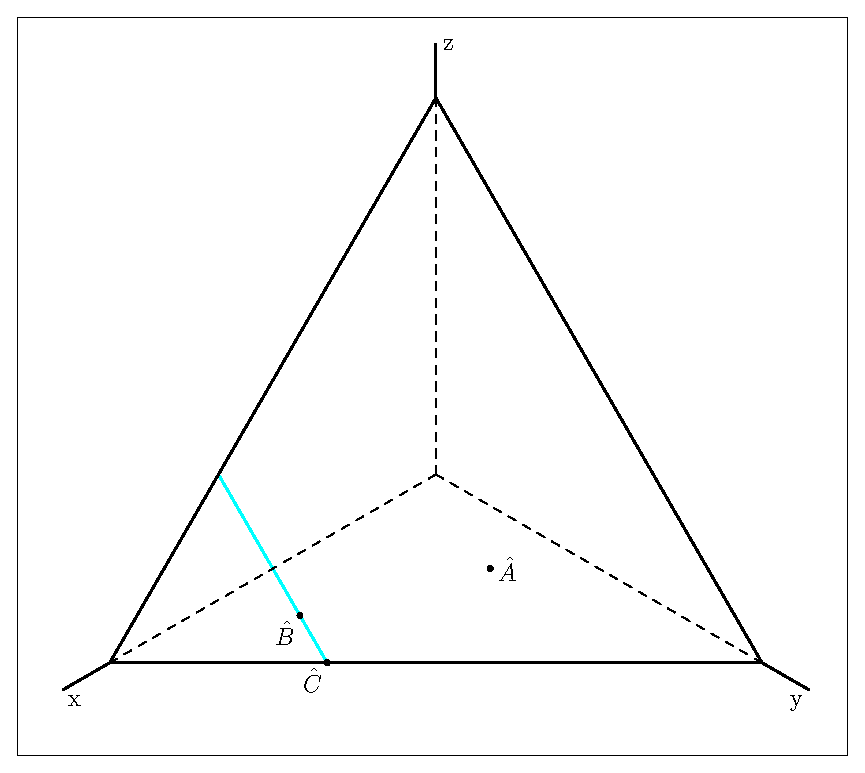
\includegraphics[scale=.6]{./threepointshat.eps}
  \end{figure}
\end{frame}

\begin{frame}
  \frametitle{Asymmetry Violation II}
  If $I(b',\omega)=I(b'',\omega)$, then for any $\lambda\in{}[0,1]$
  one has\newline
  $I(\lambda{}b'+(1-\lambda)b'',\omega)=I((1-\lambda){}b'+\lambda{}b''),\omega)$.
\end{frame}

\begin{frame}
  \frametitle{Asymmetry Violation III}
  \begin{figure}[h]
    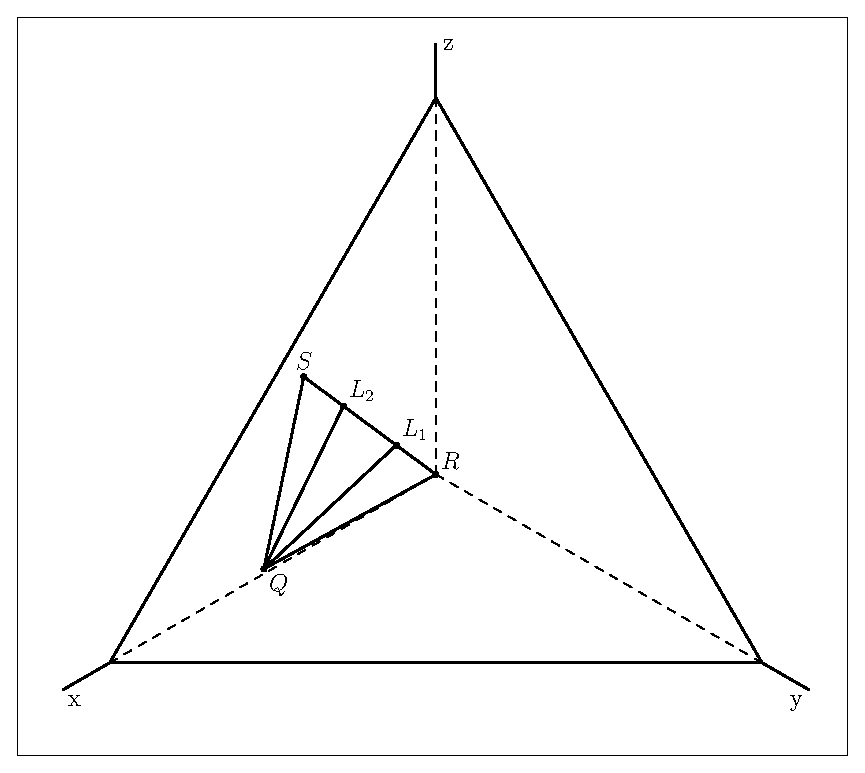
\includegraphics[scale=.6]{./symmetrylp.eps}
  \end{figure}
\end{frame}

\begin{frame}
  \frametitle{Asymmetry Violation IV}
  \begin{figure}[h]
    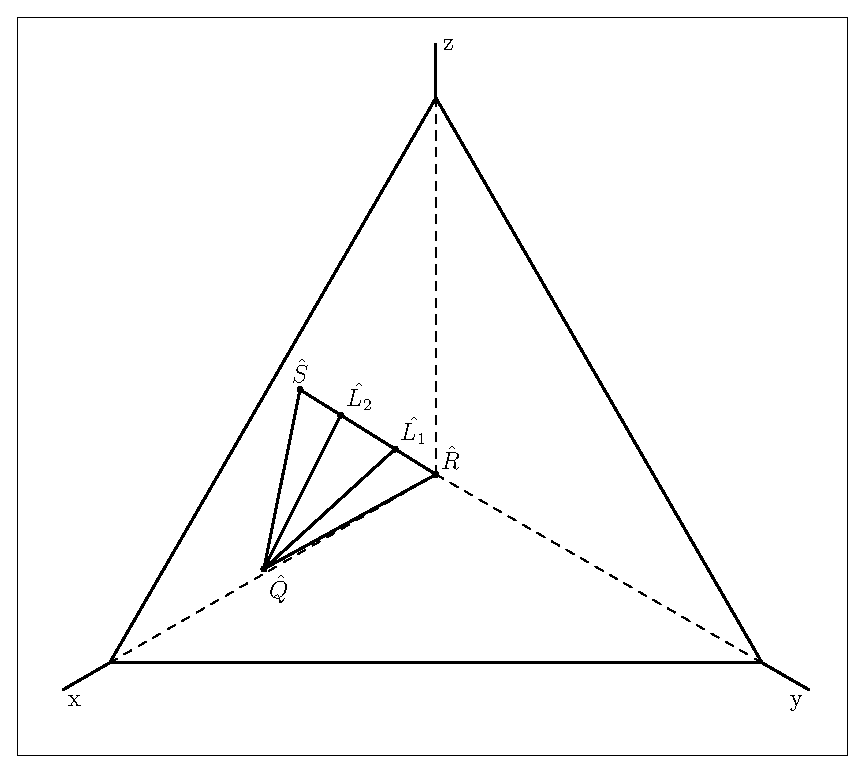
\includegraphics[scale=.6]{./symmetryrj.eps}
  \end{figure}
\end{frame}

\begin{frame}
  \frametitle{Asymmetry Violation V}
  \begin{figure}[h]
    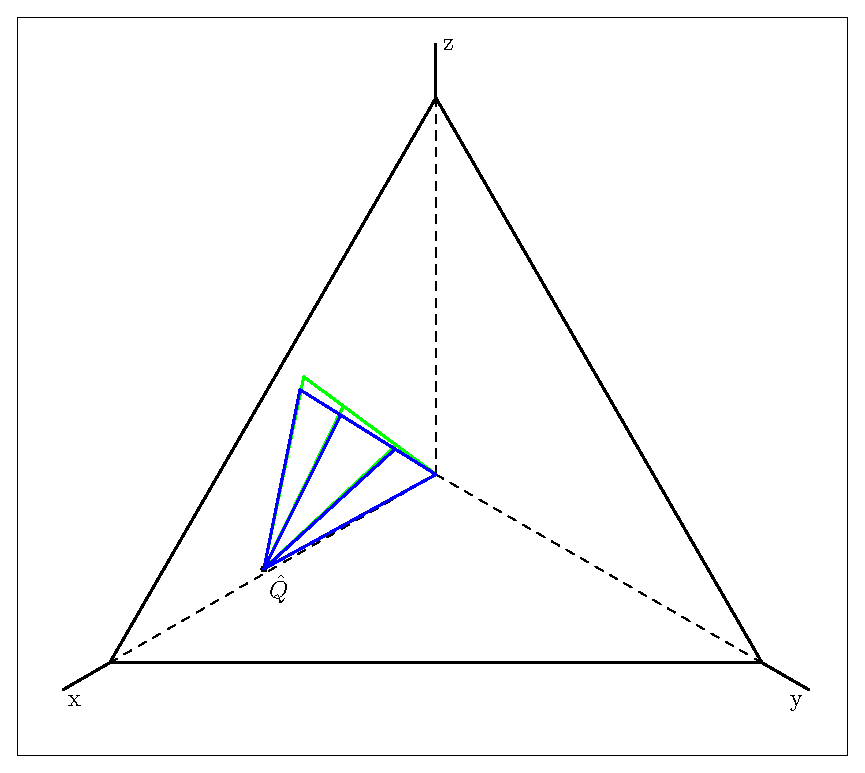
\includegraphics[scale=.6]{./symmetrytgr.eps}
  \end{figure}
\end{frame}

\begin{frame}
  \frametitle{End of Presentation}
Thank you for your attention.
\end{frame}

\end{document}